\centerline{\Large\bfseries Code Performance \& Resource Costs}

Since our software is an MPI library, its performance does not decide the resource needs.
Instead, the application or benchmark programs used in our evaluation will decide the resource
requirement. The nature of the research requires us to run different benchmarks and in different
system configurations such as different numbers of ranks per node and different numbers of total
ranks. Additional, we sometimes needs to leave some cores in each node unuse (by the MPI) to
properly evaluate the performance. All of these making the estimation of the resources required
very challenging.

The XSEDE resources will mainly be used in medium (500-1000 cores) and large
(1000+ cores) runs. We have used a startup allocation of 50,000 SUs (TG-ECS190004) to perform
preliminary evaluation of CryptMPI using micro-benchmarks, and
NAS parallel benchmarks (Class D on 784-ranks on 112-nodes). In this project period, we plan to
run NAS parallel benchmarks, Class E on a larger number of nodes as well as MPI applications
and benchmarks such as CORAL benchmark codes would take longer time. 

In the following, we will report performance results with ping-pong, OSU benchmarks, stencil
benchmarks, and NAS parallel benchmarks that we obtained on
PSC Bridges (regular memory), which compare three MPI libraries: the traditional unencrypted
MPI ($Unencrypted$), a naive implementation ($Naive$), and CryptMPI. 

\noskipheading{Ping Pong.}
The ping-pong results on Bridges are shown in \figref{fig:xsede_pingpong}. Because of
the low of computation power, the naive approach has very high overhead on Bridges.
For instance, with 4MB message size,
the $naive$ approach's overhead is 754.87\% compared to the $unencrypted$
base. On the other hand, by using pipelining and multi-threading, CryptMPI performs
518.93\% better than Naive.

\begin{figure}[htb]
	\centering
		\includegraphics[width=0.4\textwidth]{graphs/infini-xsede-pingpong.eps}
	\caption{Average %unidirectional 
	ping-pong throughput on PSC Bridges.}
	\label{fig:xsede_pingpong}
	\vspace{-2ex}
\end{figure}

\heading{OSU Multiple-Pair bandwidth.}
The multi-pair results on Bridge, Omni-path are shown in
\figref{fig:xsede_multipair_infiniband}.
All three libraries have similar
performance when there are a sufficient number of pairs of communication.
However, when the message size is small and there are only a small number
of concurrent flows, the relative speed between encryption and communication
has a larger impact. When the number of concurrent pairs is small,
even for large messages, $\Naive$ has very high overheads. For instance in
two pairs for 4MB messages the overhead for $\Naive$  is 178.48\% and
for CryptMPI is 5.03\%: $\sysrm$ again consistently performs
better than $\Naive$ due to the optimization techniques incorporated.


\heading{Stencil Kernels.}
We run 784-rank Stencil kernels on 112 nodes. 
The results for 2D stencil with different computation loads
are illustrated in~\figref{fig:2d_stencil}. 
%To see the trends more clearly, we compare the communication time, 
%instead of the total time. 
When the computational load is not heavy then CryptMPI
significantly improves the performance of the naive  approach. 
For example, for 60\% load and 2MB messages, 
the encryption overhead in CryptMPI is 206\%, 
whereas that of the naive approach is 331\%. 
Even when computational load is heavy---an unfavorable condition for CryptMPI, 
the improvement of CryptMPI over the naive approach is still noticeable. 
For example, under 80\% computational load and 256KB messages, CryptMPI's
encryption overhead is 384\%, 
whereas that of the naive approach is 450\%.
This indicates that the optimization techniques in CryptMPI
are effective for this type of applications. 


\begin{figure}[hbp]
\centering
	\subfloat[$64$KB-messages]{
	  \includegraphics[width=0.4\textwidth]{graphs/infini-multi-pair-xsede-64KB.eps}%
	}
\subfloat[$4$MB-messages]{
	  \includegraphics[width=0.4\textwidth]{graphs/infini-multi-pair-xsede-4MB.eps}%
	}
	\captionsetup{singlelinecheck=false}
	\caption{OSU Multiple-Pair throughput on PSC Bridges. }
	\label{fig:xsede_multipair_infiniband}
	\vspace{-1.5ex}
	%\end{figure}
	\end{figure}


\begin{figure}[htbp]	
	\centering
	\subfloat[$256$KB-messages]{
	  \includegraphics[width=0.32\textwidth]{graphs/2d-256KB.eps}%
	}
	\subfloat[$2$MB-messages]{
	  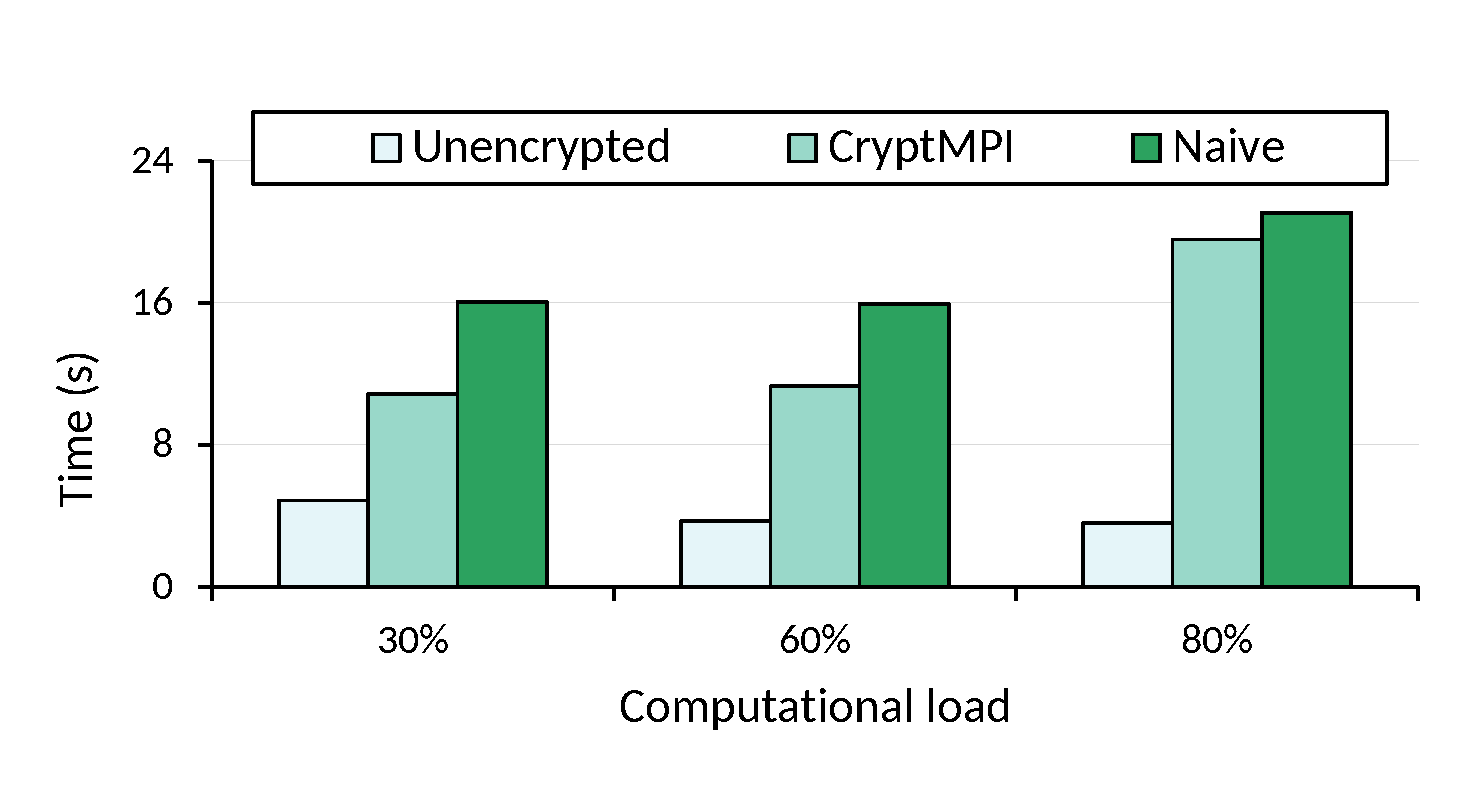
\includegraphics[width=0.32\textwidth]{graphs/2d-2MB.eps}%
	}
	\captionsetup{singlelinecheck=false}
	\caption{2D Stencil communication time, for 784-rank and 112-node, PSC Bridges.}
	\label{fig:2d_stencil}
	\vspace{-1.5ex}
	%\end{figure}
	\end{figure}


\heading{NAS benchmarks.} %Our large runs for NAS benchmarks on PSC Bridges have not completed as the time of this writing,
%and thus we are unable to report them at this time. 
{
NAS benchmarks (CG, LU, SP, BT)
timings on PSC Bridges are shown in Table~\ref{tab:NAS_PSC_INTER_NODE}.
We ran CG with 512 ranks and 128 nodes because CG can only run with the power of 2 ranks.
The rest of the programs were run with 784 ranks and 112 nodes. 
Since $\sysrm$ only optimizes the inter-node communication that requires encryption,
we compare the total inter-node communication time, total communication time, and total
application time. CryptMPI's improvement over $Naive$ varies from one benchmark to another.
For instance, the total execution time
overhead of CG for the $\sysrm$ is $20.2\%$ and for the $\Naive$ approach is $39.69\%$,
compared with the unencrypted base. In the case of BT, where the application itself overlap
computation and communication, both $\sysrm$ and $\Naive$ approach
has a low total execution time overhead: $4.53\%$ for $\sysrm$ and $5.14\%$ for the $\Naive$
approach. In the more practical situations like
the NAS benchmarks, there are factors that can affect the effectiveness
of $\sysrm$, including the following.

\begin{itemize}
\item The current CryptMPI only improves the naive approach
  for messages of at least 64KB, and thus there might be no noticeable
    difference between the two libraries
    for applications that have largely small messages.

\item CryptMPI's approach of using multi-thread encryption is only
  beneficial if there are still some idle computational resources to
    exploit, which may not hold for some computationally intensive situations.

\item Finally, CryptMPI's pipelining will give a diminishing return if
  there is already a significant overlapping between computation and
    communication in the application. Such a situation basically hides
    the communication overheads; and both $Naive$ and CryptMPI should have
    a low overhead. This happens in the BT benchmark.
\end{itemize}
        
\begin{table*}[!tbp]
		
		\centering
		\captionsetup{justification=centering, labelsep=newline}
		\caption{{Average Inter-node Communication ($t$\textsubscript{$icom$}), Total Communication ($t$\textsubscript{$tcom$}) and Total Execution ($t$\textsubscript{$exe$}) 
		Time (seconds) of NAS Parallel Benchmarks, Class D, 784-rank and 112-node (CG 512-rank and 128-node), on PSC Bridges.}}
		{\begin{tabular}{p{0.1\linewidth}*{12}{p{0.045\linewidth}}}
		\toprule[1.25pt]
		& \multicolumn{3}{|c|}{\textbf{CG}} & \multicolumn{3}{c|}{\textbf{LU}} & \multicolumn{3}{c|}{\textbf{SP}} & \multicolumn{3}{c|}{\textbf{BT}}\\
		& $t$\textsubscript{$icom$} & $t$\textsubscript{$tcom$} & $t$\textsubscript{$exe$} & $t$\textsubscript{$icom$} & $t$\textsubscript{$tcom$} & $t$\textsubscript{$exe$} & $t$\textsubscript{$icom$} & $t$\textsubscript{$tcom$} & $t$\textsubscript{$exe$} & $t$\textsubscript{$icom$} & $t$\textsubscript{$tcom$} & $t$\textsubscript{$exe$} \\ \midrule
		\textbf{Unencrypted} & 7.77 &  13.17 & 27.09 & 6.30  & 32.11 & 52.17 & 24.67 & 35.94 & 62.40 & 26.49 & 40.54 & 69.89 \\
		\textbf{CryptMPI}  & 8.73 &  14.80 & 32.56 & 8.80  & 34.26 & 56.24 & 30.01 & 39.54 & 67.64 & 28.54 & 42.25 & 73.06 \\
		\textbf{Naive}  & 13.91 &  20.93 & 37.84 & 9.71  & 36.06 & 57.87 & 31.62 & 40.11 & 68.18 & 29.03 & 42.67 & 73.49 \\ 
		\bottomrule[1.25pt]
		\end{tabular}}
		%\caption{Average inter-node communication time (seconds) of NAS parallel benchmarks, Class D, 64-rank and 8-node, on InfiniBand.}
		\label{tab:NAS_PSC_INTER_NODE}
		
\end{table*}


